\chapter{Appendix C: Flowchart of User and System Interactions}
\label{AppendixC}

The interaction diagram of the user interacting with the system, provided input and output for subsystems, and the systems working with one another. 
    To read the flow chart, start from the top to the bottom. 
    First the user creates a network using the GUI Network Creation Tool. 
    After the graph is finished, the user provides an implementation of the network as an ODE model, using Python. 
    Once finished, the user provides the network file and ODE model to the ODE solver. 
    The solver uses information from the network file to determine the number of agents to create, parameter details (including names, values, and dimensions), and setting values.
    Then the user interacts with the Visualization Dashboard Tool, for example by clicking on buttons to run simulations, changing parameter values, (un)selecting checkboxes, and zooming in and out of plots, and hovering over plots to show data. 
    Once a user has selected the parameter values, the parameter values are sent to the solver. 
    The solver calculates the time and population values using the provided graph and ODE model and sends the data back to the Visualization Dashboard Tool, which then outputs the visualizations. 
    If the user has run an ultimate analysis, then the user can query the saved data to make their own custom visualizations.
\begin{figure}
    \centering
    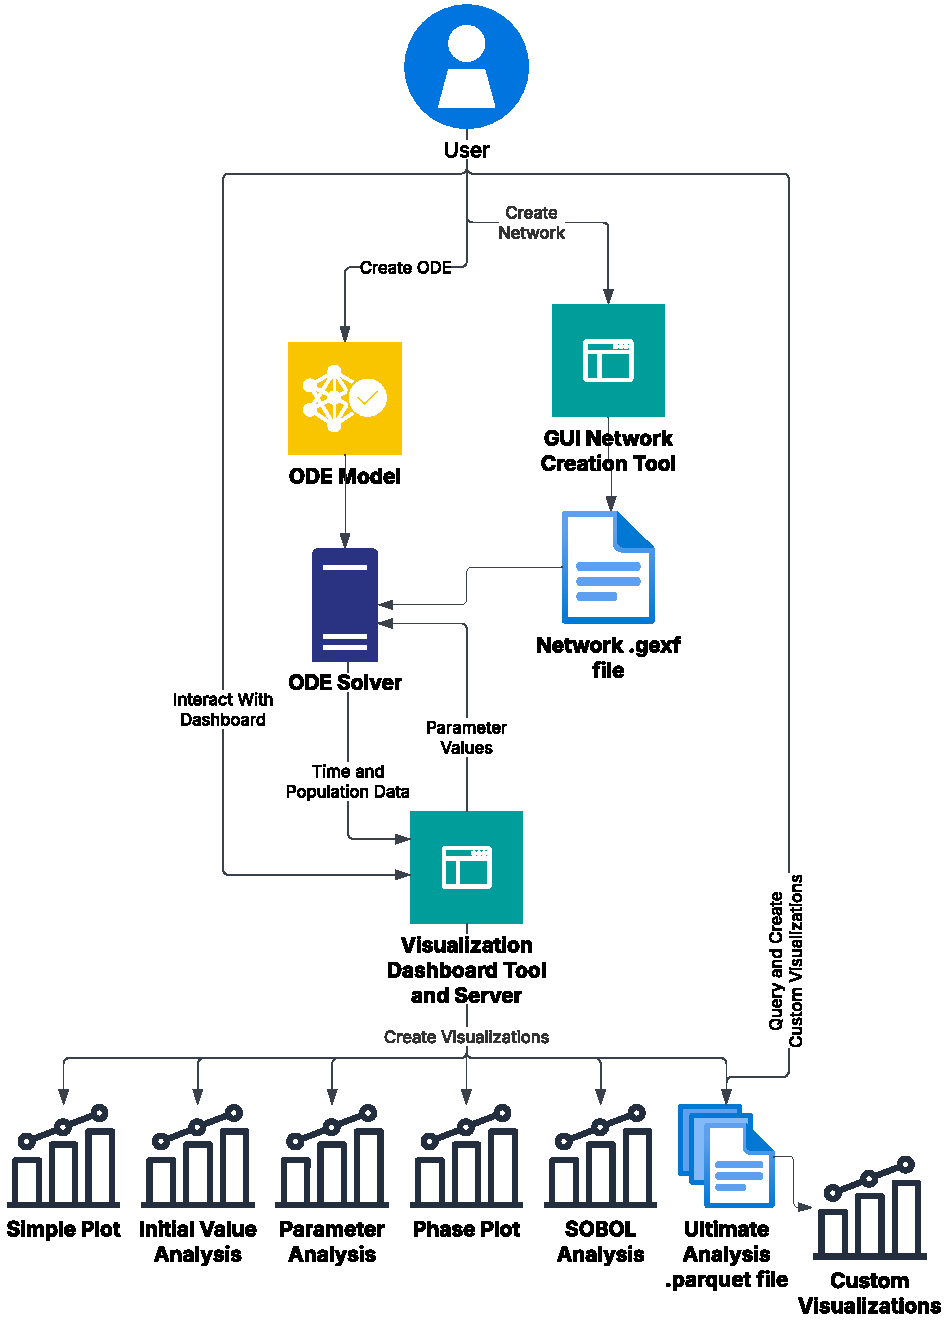
\includegraphics[width=0.8\linewidth]{Images/interaction_diagram.pdf}
    \captionsetup{width=1\linewidth}
    \caption{
        The flowchart of user and system interactions. Read from top to bottom. 
    }
    \label{fig:interaction_diagram}
\end{figure} 